%% abtex2-modelo-include-comandos.tex, v-1.9.5 laurocesar
%% Copyright 2012-2015 by abnTeX2 group at http://www.abntex.net.br/ 
%%
%% This work may be distributed and/or modified under the
%% conditions of the LaTeX Project Public License, either version 1.3
%% of this license or (at your option) any later version.
%% The latest version of this license is in
%%   http://www.latex-project.org/lppl.txt
%% and version 1.3 or later is part of all distributions of LaTeX
%% version 2005/12/01 or later.
%%
%% This work has the LPPL maintenance status `maintained'.
%% 
%% The Current Maintainer of this work is the abnTeX2 team, led
%% by Lauro César Araujo. Further information are available on 
%% http://www.abntex.net.br/
%%
%% This work consists of the files abntex2-modelo-include-comandos.tex
%% and abntex2-modelo-img-marca.pdf
%%

% ---
% Este capítulo, utilizado por diferentes exemplos do abnTeX2, ilustra o uso de
% comandos do abnTeX2 e de LaTeX.
% ---
 
\chapter{Meta-Reasoning for selection}\label{ch:rghs}

% ---
\section{Greedy Heuristic Selection (GHS)}
\noindent
We present a greedy algorithm selecction for approximately solving the heuristic subset selection problem while optimizing different objective functions. We consider the following general optimization problem.

\begin{equation}
\begin{split}
\textbf{minimize}_{\zeta\sp{'}\ \subseteq\ \zeta}\Psi(\zeta\sp{'}, \nabla) \\
\end{split}
\label{eq:equationmin}
\end{equation}

Where $\Psi(\zeta\sp{'},\nabla)$ is an objective function that we want to minimize using a subset of heuristics $\zeta\sp{'}$ that is selected from $\zeta$. According to Rayner; Sturtevant; Bowling, (\citeyear{raynersss13}) it is unlikely that there is an efficient algorithm for solving Equation \ref{eq:equationmin}.We use an algorithm based on the local search we call Greedy Heuristic Selection (\texttt{GHS}) to approximately solve Equation \ref{eq:equationmin} for different functions $\Psi$.\\

\begin{algorithm}
\SetKwInOut{Input}{Input}
\SetKwInOut{Output}{Output}
\Input{problem $\nabla$, set  of heuristics $\zeta$}
\Output{heuristic subset $\zeta\sp{'} \subseteq \zeta$}

$\zeta\sp{'} \leftarrow \emptyset$\\
%$i\ \leftarrow 0$\\ 
\While {$\Psi$ can be improved} {
	$h\ \leftarrow\ \argminA_{h \in \zeta}  \Psi(\zeta\sp{'} \cup \{h\}, \nabla)$\\
	$\zeta\sp{'} \leftarrow \zeta\sp{'} \cup \{h\}$\\
	%\If{$\Psi(\zeta_{i-1}\sp{'} \cup \{h\}$ can be improved}{
		%$\zeta_{i}\sp{'} \leftarrow \zeta_{i-1}\sp{'} \cup \{h\}$\\
		%$i++$\\
	%}	
} 
return $\zeta\sp{'}$
\caption{Greedy Heuristic Selection}
\label{alg:ghs_algorithm}
\end{algorithm}

Algorithm \ref{alg:ghs_algorithm} shows \texttt{GHS}. \texttt{GHS} receives as input a problem $\nabla$, a set of heuristics $\zeta$, and it returns a subset $\zeta\sp{'} \subseteq \zeta$. In each iteration \texttt{GHS} greedily selects from $\zeta$ the heuristics $h$ which will result in the largest reduction of the value $\Psi$ (line 3). \texttt{GHS} returns $\zeta\sp{'}$ once the objective function can not be improved. In other words, the algorithm will halt when adding another heuristic does not improve the objective function.

% --
\section{Approximately Minimizing Search Tree Size}
% ---
\noindent
The first objective function $\Psi$ we consider accounts for the number of expansions A$\sp{*}$ performs while solving a given planning problem. The planning problem must be solvable, this means $C\sp{*}$ can not be infinity. When solving $\nabla$ using the consistent heuristic function $h_{max}(\zeta\sp{'})$  for $\zeta\sp{'} \subseteq \zeta$, A$\sp{*}$ expands in the upper bound $J(\zeta\sp{'},\nabla)$ nodes, where

\begin{equation}
J(\zeta\sp{'},\nabla) = |\{s \in V | f_{max}(s,\zeta\sp{'}) \leq C\sp{*}\}|
\label{eq:eq_size_search_tree_1}
\end{equation}
\begin{equation}
J(\zeta\sp{'},\nabla) = |\{s \in V | h_{max}(s,\zeta\sp{'}) \leq C\sp{*} - g(s)\}|
\label{eq:eq_size_search_tree_2}
\end{equation}

We write $J(\zeta\sp{'})$ or simply $J$ instead of $J(\zeta\sp{'},\nabla)$. \texttt{GHS} is able to find the solutions when we use $J$ as the objective function $\Psi$.

\section{Approximately Minimizing A*'s Running Time}
\noindent
Another objective function $\Psi$ we consider accounts for the A$\sp{*}$ running time and is defined as follows. Let $T(\zeta\sp{'},\nabla)$ be an approximation to the running time of A$\sp{*}$ when using $h_{max}(\zeta\sp{'})$ for solving $\nabla$, defined as follows.

\begin{equation}
T(\zeta\sp{'}, \nabla) = J(\zeta\sp{'},\nabla) \cdot t_{h_{max}}(\zeta\sp{'})
\label{eq:eq_time_solving}
\end{equation}

where, for any heuristic function $h$, the term $t_{h}$ refers to the running time used for computing the $h-$value of any state $s$. \\

We assume that $t_{h}$ to be independent of $s$, which is a reasonable assumption for several heuristics such as \texttt{PDBs}.\\

In order to compute the running time of A$\sp{*}$ exactly we would also have to account for all nodes evaluated. Specifically, our objective function accounts for the generation time added to the heuristic evaluation time of all nodes generated, not only nodes expanded. In this way, $T(\zeta\sp{'},\nabla)$ is reasonable approximation for A$\sp{*}$'s running time for the heuristic subset selection problem.\\

\section{Estimating Tree Size and Running Time}
In  practice \texttt{GHS} used approximations models of $J,T,$ and $T\sp{'}$ instead of their exact values. This is because computing $J,T,$ and $T\sp{'}$ exactly would require solving $\nabla$. We denote the approximations of $J$ as \textit{\^{J}}, and since both $T$ and $T\sp{'}$ model A$\sp{*}$'s running time, we denote the approximation for both as \textit{\^{T}}.\\

We use the Culprit Sampler (\texttt{CS}) introduced by Barley; Franco; Riddle, (\citeyear{BarleySantiagoOver}) and the Stratified Sampling (\texttt{SS}) algorithm introduced by Chen, (\citeyear{chen1992heuristic}) for computing \textit{\^{J}} and \textit{\^{T}}. Each of the two algorithms has its strengths and weaknesses, which we explore in the experimental Chapter.\\

Both \texttt{CS} and \texttt{SS} must be able to quickly estimate the values of \textit{\^{J}}$(\zeta\sp{'})$ and \textit{\^{T}}$(\zeta\sp{'})$ for any subset $\zeta\sp{'}$ of $\zeta$ so they can be used in \texttt{GHS}'s optimization process.

\section{Culprit Sampler (CS)}
\noindent
\texttt{CS} runs a time$-$bounded A$\sp{*}$ search while sampling $f-culprits$ and $b-culprits$ to estimate the values of \textit{\^{J}} and \textit{\^{T}}.

\begin{definition}(f-culprit)
Let $\zeta = \{h_{1}, h_{2},...,h_{M}\}$ be a set of heuristics. The f$-$culprit of a node n in an A$\sp{*}$ search tree is defined as the tuple F(n) = $\left\langle f_{1}(n), f_{2}(n),...,f_{M}(n)  \right\rangle$, where $f_{i}(n) = g(n)+h_{i}(n)$. For any n$-$tuple F, the counter $C_{F}$ denotes the number of nodes n in the tree with F(n) = F.
\label{def:def_fculprits}
\end{definition}

\begin{definition}(b-culprit)
Let $\zeta = \{h_{1}, h_{2},...,h_{M}\}$ be a set of heuristics and b a lower bound on the solution cost $\nabla$. The b$-$culprit of a node n in an A$\sp{*}$ search tree is defined as the tuple $B(n) = \left\langle y_{1}(n), y_{2}(n),...,y_{M}(n)\right\rangle$, where $y_{i}(n) = 1$ if g(n) + $h_{i}(n) \leq b$ and $y_{i}(n) = 0$, otherwise.  For any binary n$-$tuple B, the counter $C_{B}$ denotes the number of nodes n in the tree with B(n) = B.
\label{def:def_bculprits}
\end{definition}

\texttt{CS} works by running an A$\sp{*}$ search bounded by a user$-$specified time limit. Then, \texttt{CS} compresses the information obtained in the A$\sp{*}$ search (\textsf{i.e.,} the $f-$values of all nodes expanded according to all heuristics $h$ in $\zeta$) in b$-$culprits, which are later used for computing \textit{\^{J}}. The b$f-$culprits are generated as an intermediate step for computing the b$-$culprits, as we explain below. The maximum number of f$-$culprits and b$-$culprits in an A$\sp{*}$ search tree is equal to the number of nodes in the tree expanded by the time$-$bounded A$\sp{*}$ search. However, in practice the number of f$-$culprits is usually much lower than the number of nodes in the tree. Moreover, in practice, the total number of different b$-$culprits tends to be even lower than the total number of f$-$culprits. Given a planning problem $\nabla$ and a set of heuristics $\zeta$, \texttt{CS} samples the A$\sp{*}$ search tree as follows.

\begin{enumerate}
    \item[1.-] \texttt{CS} runs A$\sp{*}$ using $h_{min}(s,\zeta) = min_{h \in \zeta}h(s)$ until reaching a user$-$specified time limit. A$\sp{*}$ using $h_{min}$ expands node $n$ if it were to expand $n$ while using any of the heuristics in $\zeta$ individually. For each node $n$ expanded in this time$-$bounded search we store $n$'s f$-$culprit and its counter.
    \item[2.-] Let $f_{maxmin}$ be the largest $f-$value according to $h_{min}$ encountered in the time$-$bounded A$\sp{*}$ search described above. We now compute the set $\mathbb{B}$ of b$-$culprits and their counters based on the f$-$culprits and on the value of $f_{maxmin}$. This is done by iterating over all f$-$culprits once.\\

\end{enumerate}
    
The process described above is performed only once \texttt{GHS}'s execution. The value of \textit{\^{J}}$(\zeta\sp{'},\nabla)$ for any subset $\zeta\sp{'}$ of $\zeta$ if then computed by iterating over all b$-$culprits \textbf{B} and summing up the relevant values of $C_{B}$. The relevant values of $C_{B}$ represent the number of nodes A$\sp{*}$ would expand in a search bounded by $b$ if using $h_{max}(\zeta\sp{'})$. This computation can be written as follows.\\

\begin{equation}
\textit{\^{J}}(\zeta\sp{'},\nabla) = \sum_{\mathbb{B} \in B}W(B)
\label{eq:eq_comp_w}
\end{equation}

Where $W(B)$ is 0 if there is a heuristic in $\zeta\sp{'}$ whose $y$-value in $B$ is zero (\textsf{i.e.,} there is a heuristic in $\zeta\sp{'}$ that prunes all nodes compressed into $B$), and $C_{B}$ otherwise. If the time$-$bounded A$\sp{*}$ search with $h_{min}$ expands all nodes $n$ with $f(n) \leq C\sp{*}$, then \textit{\^{J}}$=J$. In practice, however, our estimate \textit{\^{J}} will tend to be much lower than $J$.\\

The value of \textit{\^{T}} is computed by multiplying \textit{\^{J}} by the sum of the evaluation time of each heuristic in $\zeta\sp{'}$. The evaluation time of the heuristics in $\zeta\sp{'}$ is measured in a separate process, before executing \texttt{CS}, by sampling a small number of nodes from $\nabla$'s start state.

\section{Stratified Sampling (SS)}
Chen, (\citeyear{chen1992heuristic}) presented a method for estimating the search tree size of backtracking search algorithms by using a stratification of the search tree to guide its sampling. We define Chen’s stratification as a type system. In the figure \ref{fig:ss_ts} each state of the search space is mapped to the \textit{Type System}.

\begin{figure}[htb]
\centering 
\begin{tikzpicture}

% -- center, xdim, ydim
\draw[very thick,cyan] \boundellipse{-2,0}{2}{4};
\draw[very thick,cyan] \boundellipse{6,0}{1}{2};
	
  % First, define nodes
% -- points F  
  
  \draw (-2,3) node[circle, inner sep=0.8pt, fill=cyan, label={{}}] (E) {};  
  \draw (6,1) node[circle, inner sep=0.8pt, fill=cyan, label={{}}] (F) {}; 

  \draw[very thick,cyan, ->>]  (E) .. controls +(5,-3) and +(-4,1).. (F);
  \path  ($(E)+(0,0.2)$) .. controls +(5,-3) and +(-4,1)..  ($(F)+(0,0.2)$) 
     {\foreach \i in {1,...,40} {  coordinate[pos=0.15+0.75*\i/40] (p\i) } };

  \draw (-1,2) node[circle, inner sep=0.8pt, fill=cyan, label={{}}] (A) {};
  \draw[very thick,cyan, ->>]  (A) .. controls +(5,-3) and +(-4,1).. (F);
  \path  ($(A)+(0,0.2)$) .. controls +(5,-3) and +(-4,1)..  ($(F)+(0,0.2)$) 
     {\foreach \i in {1,...,40} {  coordinate[pos=0.15+0.75*\i/40] (p\i) } };
	
  \draw (-3,0) node[circle, inner sep=0.8pt, fill=cyan, label={{}}] (B) {};
  \draw[very thick,cyan, ->>]  (B) .. controls +(5,-3) and +(-4,1).. (F);
  \path  ($(B)+(0,0.2)$) .. controls +(5,-3) and +(-4,1)..  ($(F)+(0,0.2)$) 
     {\foreach \i in {1,...,40} {  coordinate[pos=0.15+0.75*\i/40] (p\i) } };
	
% -- points in G

  \draw (-2,1) node[circle, inner sep=0.8pt, fill=cyan, label={{}}] (C) {};
  \draw (6.5,0) node[circle, inner sep=0.8pt, fill=cyan, label={{}}] (G) {};
  \draw[very thick,cyan, ->>]  (C) .. controls +(5,-3) and +(-4,1).. (G);
  \path  ($(C)+(0,0.2)$) .. controls +(5,-3) and +(-4,1)..  ($(G)+(0,0.2)$) 
     {\foreach \i in {1,...,40} {  coordinate[pos=0.15+0.75*\i/40] (p\i) } };	

\draw (-1,0) node[circle, inner sep=0.8pt, fill=cyan, label={{}}] (D) {};	
\draw[very thick,cyan, ->>]  (D) .. controls +(5,-3) and +(-4,1).. (G);
  \path  ($(C)+(0,0.2)$) .. controls +(5,-3) and +(-4,1)..  ($(G)+(0,0.2)$) 
     {\foreach \i in {1,...,40} {  coordinate[pos=0.15+0.75*\i/40] (p\i) } };	

\draw (-3,-1) node[circle, inner sep=0.8pt, fill=cyan, label={{}}] (H) {};	
\draw[very thick,cyan, ->>]  (H) .. controls +(5,-3) and +(-4,1).. (G);
  \path  ($(C)+(0,0.2)$) .. controls +(5,-3) and +(-4,1)..  ($(G)+(0,0.2)$) 
     {\foreach \i in {1,...,40} {  coordinate[pos=0.15+0.75*\i/40] (p\i) } };
	
% -- X
\draw (-2,-2) node[circle, inner sep=0.8pt, fill=cyan, label={{}}] (J) {};
  \draw (6,-1) node[circle, inner sep=0.8pt, fill=cyan, label={{}}] (X) {};
  \draw[very thick,cyan, ->>]  (J) .. controls +(5,-3) and +(-4,1).. (X);
  \path  ($(C)+(0,0.2)$) .. controls +(5,-3) and +(-4,1)..  ($(G)+(0,0.2)$) 
     {\foreach \i in {1,...,40} {  coordinate[pos=0.15+0.75*\i/40] (p\i) } };

\draw (-2,-3) node[circle, inner sep=0.8pt, fill=cyan, label={{}}] (K) {};
\draw[very thick,cyan, ->>]  (K) .. controls +(5,-3) and +(-4,1).. (X);
  \path  ($(C)+(0,0.2)$) .. controls +(5,-3) and +(-4,1)..  ($(G)+(0,0.2)$) 
     {\foreach \i in {1,...,40} {  coordinate[pos=0.15+0.75*\i/40] (p\i) } };

$\node [xshift=1cm,yshift=2cm] (A) at (-3,3) {Search Space};$

$\node [xshift=1cm,yshift=2cm] (A) at (5,1) {Type System};$
	
\end{tikzpicture}
\caption{Type system and the search space representation.} \label{fig:ss_ts}
\end{figure}

\subsection{Type System}
The \textit{Type System} is a partition of the states in the state space and it is calculated based of any property of each node in the search tree. Lelis, (\citeyear{Lelis2013CC})

A common mistake about \textit{type system} is to think that it is an abstraction of the state$-$space. Prieditis, (\citeyear{Prieditis93}) defines a state$-$space abstraction as a simplified version of the problem where:
\begin{itemize}
\item The cost of the least$-$cost path between two abstracted states must less than or equal to the cost of the least$-$cost path between the corresponding two states in the original state$-$space.
\item Goal states in the original state$-$space must be goal states in the abstracted state$-$space.
\end{itemize}

The difference between state$-$space abstractions and \textit{type system} is that the last one does not have the two requeriments mentioned above. Also, there is not relation between types to argue that the \textit{type system} can be represented as a graph. Furthermore, the relation between \textit{type system} and abstractions is that \textit{type system} can not necessarily used as abstractions, and abstraction always can be used as a \textit{type system} Prieditis, (\citeyear{Prieditis93}).\\

\begin{definition}{Type System}
Let S = (N,E) be a search tree, where N is its set of nodes and  for each n $\in$ N, $\{n\sp{'}|(n,n\sp{'})\ \in\ E \}$ is n's set of child nodes. $TS = \{t_{1},...,t_{k} \}$ is a type system for S if it is a disjoint partitioning of N. If $n\ \in\ N$ and $t\ \in\ TS$ with $n\ \in\ t$, we write $TS(n) = t$.
\end{definition}

\texttt{SS} is a general method for approximating any function of the form $\varphi = \sum_{n \in S}z(n)$, where $z$ is any function assigning a numerical value to a node.  $\varphi$ represents a numerical property of the search tree rooted at $n\sp{*}$. For instance, if $z(n)=1$ for all $n \in S$, then $\varphi$ is the size of the tree.\\

Instead of traversing the entire tree and summing all $z-$values, \texttt{SS} assumes subtrees rooted at nodes of the same type will have equal values of $\varphi$ and only one node of each type, chosen randomly, is expanded. This is the key to $\texttt{SS}$'s efficiency since the search trees of practical interest have far too many nodes to be examined examined exhaustively.\\

Given a search tree $S$ and a type system $TS$, \texttt{SS} estimates $\varphi$ as follows. First, it samples the tree and returns a set $A$ of $representative-weight$ pairs, with one such pair for every unique type seen during sampling. In the pair $\left\langle s,w \right\rangle$ in $A$ for type $t \in TS$, $n$ is the unique node of type $t$ that was expanded during search and $w$ is an estimate of the number of nodes type $t$ in the tree. $\varphi$ is then approximated by $\hat{\varphi}$, defined as, $\hat{\varphi} =  \sum_{\left\langle s,w \right\rangle \in A}w \times z(n)$.\\

By making $z(n) = 1$ for all $n \in S$ \texttt{SS} prooduces an estimate $\hat{J}$ of $J$. Similarly to our approach with \texttt{CS}, we obtain $\hat{T}$ by multiplying $\hat{J}$ by the heuristic evaluation time.


\begin{algorithm}
\SetKwInOut{Input}{Input}
\SetKwInOut{Output}{Output}
\Input{root $n\sp{*}$ of a tree and a type system $T$}
\Output{an array of sets $A$, where $A[i]$ is the set of pairs $<n,w>$ for the nodes $n$ expanded at level $i$.}

$A[0] \leftarrow \{\left\langle  n\sp{*},1 \right\rangle \}$

$i \leftarrow 0$

\While{A[i] is not empty} {
	\For{each element $\left\langle n,w \right\rangle$ in $A[i]$} {
		\For{each child $\hat{n}$ of n} {
			\If{$g(\hat{n}) + h(\hat{n}) \leq d$} {
				\If{$A[i+1]$ contains an element $\left\langle n\sp{'}, w\sp{'} \right\rangle$ with $T(n\sp{'}) = T(\hat{n})$} {
				$w\sp{'} \leftarrow w\sp{'} + w$\\ 
				with probability $w/w\sp{'}$, replace $\left\langle n\sp{'}, w\sp{'} \right\rangle$ in\\ $A[i+1]$ by $\left\langle \hat{n},w\sp{'} \right\rangle$
				} \Else {	
					insert new element $\left\langle \hat{n},w\sp{'} \right\rangle$	 in $A[i+1]$
				}
			}
		}
	}
	$i \leftarrow i + 1$
}
\caption{SS, a single probe}
\label{alg:ss_algorithm}
\end{algorithm}

In \texttt{SS} the types are required to be partially ordered: a node's type must be strictly greater than the type of its parent. This can be guaranteed by adding the depth of a node to the type system and then sorting the types lexicographically. That is why in our implementation of \texttt{SS} types at one level are treated separately from types at another level by the division of $A$ into groups $A[i]$, where $A[i]$ is the set of representative$-$weight pairs for the types encountered at level $i$. If the same type occurs on differente levels the occurrences will be treated as if they were different types $-$ the depth of search is implicitly included into all of our type systems.\\

Algorithm \ref{alg:ss_algorithm} shows \texttt{SS} in detail. Representative nodes from $A[i]$ are expanded to get representative nodes for $A[i+1]$ as follows. $A[0]$ is initialized to contain only the root of the search tree to be probed, with weight 1 (Line 1). In each iteration (Lines 4 through 11), all nodes in $A[i]$ are expanded. The children of each node in $A[i]$ are considered for inclusion in $A[i+1]$ if their $f-$value do not exceed an upper bound $d$ provided as input to \texttt{SS}. If a child $\hat{n}$ has a type $t$ that is already represented in $A[i+1]$ by another node $n\sp{'}$, then a $merge$ action on $\hat{n}$ and $n\sp{'}$ is performed. In a merge action we increase the weight in the corresponding representative$-$weight pair of type $t$ by the weight $w(n)$ of $\hat{n}$'s parent $n$ (from level $i$) since there were $w(n)$ nodes at level $i$ that are assumed to have children of type $t$ at level $i+1$. $\hat{n}$ will replace $n\sp{'}$ according to the probability shown in Line 9. Chen, (\citeyear{chen1992heuristic}) proved that this probability reduces the variance of the estimation. Once all the states in $A[i]$ are expanded, we move to the next iteration.\\

One run of the \texttt{SS} algorithm is called a $probe$. Chen,  (\citeyear{chen1992heuristic}) proved that the expected value of $\hat{\varphi}$ converges to $\varphi$ in the limit as the number of probes goes to infinity. As Lelis; Stern; Sturtevant,  (\citeyear{lelis2014estimating}), \texttt{SS} is not able to detect duplicated nodes in its sampling process. As a result, since A$\sp{*}$ does not expanded duplicates, \texttt{SS} usually overestimates the actual number of nodes A$\sp{*}$ expands. Thus, in the limit, as the number of probes grows large, \texttt{SS}'s prediction converges to a number which  is likely to overestimate the A$\sp{*}$ search tree size. We test empirically whether \texttt{SS} is able to allow \texttt{GHS} to make near-optimal subset selection with respect to A$\sp{*}$ search tree in 10\% optimal and good subset selection with respect to the A$\sp{*}$ running time, despite being unable to detect duplicated nodes during sampling.\\

Similarly to \texttt{CS}, we also define a time$-$limit to run \texttt{SS}. We use \texttt{SS} with an iterative$-$deepening approach in order to ensure an estimate of $\hat{J}$ and $\hat{T}$ before reaching the time limit. We set the upper bound $d$ to the heuristic value of the start state and, after performing $p$ probes, if there is still time, we increase $d$ to twice its previous value. The values of $\hat{J}$ and $\hat{T}$ is given by the prediction produced for the last $d-$value in which \texttt{SS} was able to perform all $p$ probes.\\

\texttt{SS} must also be able to estimate the values of $\hat{J}(\zeta\sp{'})$ and $\hat{T}(\zeta\sp{'})$ for any subset $\zeta\sp{'}$ of $\zeta$. This is achieved by using \texttt{SS} to estimate b$-$culprits (See Definition \ref{def:def_bculprits}) instead of the search tree size directly. Similarly to \texttt{CS, SS} used $h_{min}$ of the heuristics in $\zeta$ to decide when to prune a node (See Line 6 of Algorithm \ref{alg:ss_algorithm}) while sampling. This ensures that \texttt{SS} expands a node $n$ if A$\sp{*}$ employing at least one of the heuristics in $\zeta$ would expand $n$ according to bound $d$. The $C_{B}$ counter of each b$-$culprit $B$ encountered during $SS$'s probe is given by,

\begin{equation}
C_{B} = \sum_{\left\langle n,w \right\rangle \in A \wedge B(n) = B}w
\label{eq:eq_CB}
\end{equation}

We recall that to compute $B(n)$ for node $n$ one needs to define a bound $b$. Here we use the bound $d$ used by \texttt{SS}. The average value of $C_{B}$ across $p$ probes is used to predict the search tree size for a given subset $\zeta\sp{'}$. As explained for \texttt{CS}, this can be done by traversing over all b$-$culprits once.\\

\if false

\section{8-tile-puzzle Case Using type system}
\noindent
In this dissertation we use \textit{type system} based only in heuristics.\cite{zahavi2010predicting} use the simpliest heuristic$-$based \textit{type system} in which two nodes $n$ and $n\sp{'}$ are of the same type if they have the same heuristic value. \\

\begin{figure}[htb]
\centering
\begin{forest}
 [\usebox\myboxc \hspace*{1.4in} \usebox\myboxb]
\end{forest}
\caption{The heuristic value is the position of the empty tile in a specific state.} \label{fig:type_system}
\end{figure}

Let's explain how \textit{type system} works through an example. The problem of 8$-$tile$-$puzzle in the Figure \ref{fig:type_system}, the center tile is labeled with the letter \texttt{M}, the corners labeled with \texttt{C} and the mediums with \texttt{E}. For this problem, we can define the \textit{type system} based on the position of the empty tile regarding the position of the empty tile in the goal state. For this case, two nodes $n$ and $n\sp{'}$ would be of the same type if $n$ and $n\sp{'}$ have the empty tile with the same letter and with the same distance to the empty tile of the goal state.\\

In the Figure \ref{fig:empty_space_ts}, each row represent a type. The first board shows the empty tile in the center with distance to the empty tile in the goal state equal to 2. The shortest path to get to the empty tile in the goal state would be doing: down$-$left or right$-$down. Which both moves represent the same cost. Then, the type would be (2,\texttt{M}). In the next board, the empty tile is in the left top, and use the letter \texttt{C}. The minimum distance is 4 because to get the goal empty tile is necessary to do: down$-$down$-$right$-$right or right$-$right$-$down$-$down, etc. So the type would be (4, \texttt{C}). In the next board, there are two tiles that have the same type, because both have the same letter \texttt{M} with distance equal to 3. Then, both have the type (3,E). The fourth row have two boards with the same type, because both have the same letter \texttt{C} with distance equal to 2. Then, both have the type (2, \texttt{C}). The fifth row have two boards with the same type, because both have the same letter \texttt{E} with distance equal to 1. Then, both have the type (1, \texttt{E}). In the last row the empty tile is in the goal empty tile. So, the distance is zero and the letter is \texttt{C}. The type would be (0, \texttt{C}).

% print types
\begin{figure}[htb]
\centering
\begin{forest}
 [\usebox\myboxcenter]
 $\node [xshift=1cm,yshift=2cm] (A) at (2,0) {(2, M)};$
\end{forest}

\begin{forest}
 [\usebox\myboxcornerone]
 $\node [xshift=1cm,yshift=2cm] (A) at (2,0) {(4, C)};$
\end{forest}

\begin{forest}
 [\usebox\myboxmediumleft \hspace*{0.2in} \usebox\myboxmediumup]
 $\node [xshift=1cm,yshift=2cm] (A) at (4,0) {(3, E)};$
\end{forest}

\begin{forest}
 [\usebox\myboxcornerthree \hspace*{0.2in} \usebox\myboxcornertwo]
 $\node [xshift=1cm,yshift=2cm] (A) at (4,0) {(2, C)};$
\end{forest}

\begin{forest}
 [\usebox\myboxmediumdown \hspace*{0.2in} \usebox\myboxmediumright]
 $\node [xshift=1cm,yshift=2cm] (A) at (4,0) {(1, E)};$
\end{forest}

\begin{forest}
 [\usebox\myboxcornerfour]
 $\node [xshift=1cm,yshift=2cm] (A) at (2,0) {(0, C)};$
\end{forest}
\caption{Each row has one or two states that represent the same type.} \label{fig:empty_space_ts}
\end{figure}

\fi

\section{SS step by step}
\noindent
% -- Explaining Stratified Sampling
In the Figure \ref{fig:ts_search_tree}, we can see how \textit{Type System} works. In the Level 1, we have the root node, the $w$ initialized with one. Let's suppose that three nodes are generated by the root node in the Level 2. The nodes in the Level 2 have the following types: red, blue and red from left to right respectively, and each node receive the same $w$ of the father. In the Level 2 we apply \texttt{SS}'s assumption, two nodes in the same level that have the same type (The same color) root subtrees of the same size and only one node of each type must be chosen randomly to be expanded. There are two nodes with type red in Level 2. In that way, we choose randomly one of them. Let's suppose we choose the right red node. Then, we have to update the number of nodes with the type red using the $w$, both red node types have $w=1$, then we sum the $w$ and the new $w=2$. As a result, in the Level 2 we will have two nodes of red type and one node with blue type. \\

\begin{figure}[htb]
\centering
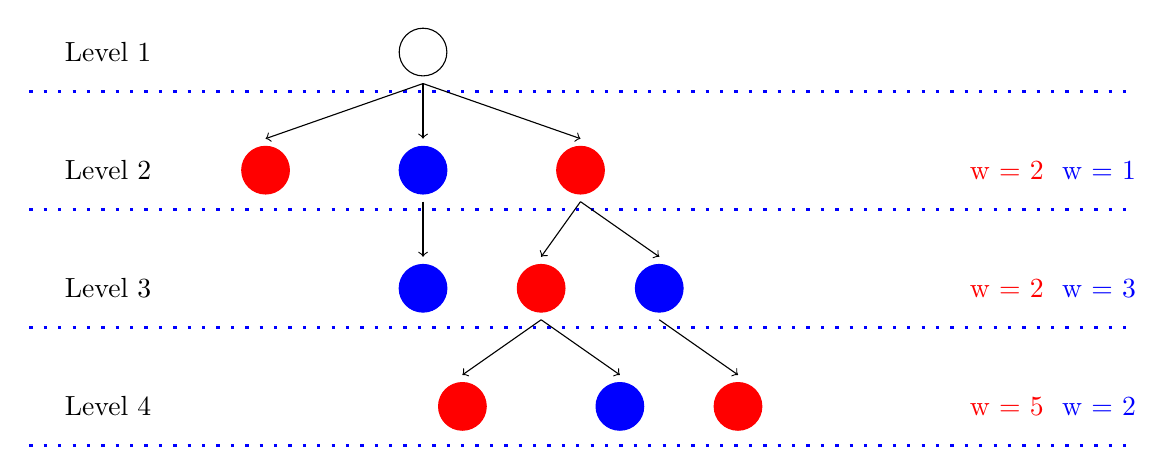
\begin{tikzpicture}

\draw[very thick,blue,loosely dotted] (-2,0) -- (12,0);
\draw[very thick,blue,loosely dotted] (-2,-1.5) -- (12,-1.5);
\draw[very thick,blue,loosely dotted] (-2,-3) -- (12,-3);
\draw[very thick,blue,loosely dotted] (-2,-4.5) -- (12,-4.5);

\node [xshift=1cm,yshift=2cm] (A) at (-2,-1.5) {Level 1};
\node [xshift=1cm,yshift=2cm] (A) at (-2,-3) {Level 2};
\node [xshift=1cm,yshift=2cm] (A) at (-2,-4.5) {Level 3};
\node [xshift=1cm,yshift=2cm] (A) at (-2,-6) {Level 4};

% -- level 1
\draw[black,fill=white] (3,0.5) circle (2ex);

% -- level 2
\draw[red,fill=red] (1,-1) circle (2ex);
\draw[blue,fill=blue] (3,-1) circle (2ex);
\draw[red,fill=red] (5,-1) circle (2ex);

% -- level 3
\draw[blue,fill=blue] (3,-2.5) circle (2ex);
\draw[red,fill=red] (4.5,-2.5) circle (2ex);
\draw[blue,fill=blue] (6,-2.5) circle (2ex);

% -- level 4
\draw[red,fill=red] (3.5,-4) circle (2ex);
\draw[blue,fill=blue] (5.5,-4) circle (2ex);
\draw[red,fill=red] (7,-4) circle (2ex);

% -- draw arrows
\draw[->] (3,0.1) -- (1,-0.6);
\draw[->] (3,0.1) -- (3,-0.6);
\draw[->] (3,0.1) -- (5,-0.6);

\draw[->] (3,-1.4) -- (3,-2.1);

\draw[->] (5,-1.4) -- (4.5,-2.1);
\draw[->] (5,-1.4) -- (6,-2.1);

\draw[->] (4.5,-2.9) -- (3.5,-3.6);
\draw[->] (4.5,-2.9) -- (5.5,-3.6);

\draw[->] (6,-2.9) -- (7,-3.6);

\node [xshift=1cm,yshift=2cm] (A) at (10,-3) {\textcolor{red}{w = 2 } \textcolor{blue}{w = 1}};
\node [xshift=1cm,yshift=2cm] (A) at (10,-4.5) {\textcolor{red}{w = 2 } \textcolor{blue}{w = 3}};
\node [xshift=1cm,yshift=2cm] (A) at (10,-6) {\textcolor{red}{w = 5 } \textcolor{blue}{w = 2}};
\end{tikzpicture}
\caption{Search tree using Type System} \label{fig:ts_search_tree}
\end{figure}

When nodes in the Level 2 are expanded. The blue node expands one node of type blue and the red node expands two nodes of type red and blue. The question here is how many nodes would be generated in the Level 3? The answer is: $1 \times \textcolor{blue}{blue} + 2 \times \textcolor{red}{red} + 2 \times \textcolor{blue}{blue}$. So, in the Level 3 we will have 2 nodes of red type and 3 nodes of type blue.\\ 

In the Level 3 the $w$ of the node blue would have the same $w$ of the father. The father has $w = 1$, then the child has $w = 1$. The $w$ of the red type and blue type would be 2. Once the $w$ has been updated for each node in the Level 3 we apply the \texttt{SS}'s assumption again. There are two nodes with type blue. So, we choose randomly one of them and update their $w$. Let's choose the right blue type and the updated $w$ would be 3 because 1 from the left blue type plus the 2 from the right blue type.\\

When nodes in the Level 3 are expanded. They are expanded in the following way: The red node expands two nodes of types red and blue and the blue node expands one of red type. How many nodes would be generated at Level 4, then? The answer is: $2 \times \textcolor{red}{red} + 3 \times \textcolor{red}{red} + 2 \times \textcolor{blue}{blue}$. Therefore, in the Level 4, we will have five nodes of type red and two nodes of type blue.\\

Finally, the number of nodes expanded in the search tree is obtained summing all $w$ plus one (The root node). As a result, the number of nodes expanded in the search tree would be $ 15 + 1 = 16$.\\


\if false
\section{Comparison between SS and IDA*}
\noindent
\texttt{SS} is an algorithm that estimates the number of nodes expanded performed by heuristic search algorithm seeking solutions in state space. We apply \texttt{SS} to predict the number of nodes expanded by IDA$\sp{*}$ in a given $f-$layer when using a consistent heuristics.\\

We first ran IDA$\sp{*}$ for Fast$-$Downward benchmark for optimal domains. Our evaluation metric is coverage, \texttt{i.e.,} number of problems solved within 30 minutes time limit. We note that in 30 minutes non all the instances for a specific domain using a consistent heuristic can be solved. Afterwards, run \texttt{SS} using as a threshold the $f-$layer for each instance of each domain, this process is executed using different number of probes \texttt{i.e.,} 1, 10, 100, 1000 and 5000.\\

\begin{equation}
\frac{\sum_{s\in PI} \frac{Pred(s, d) - R(s, d)}{R(s, d)}}{|PI|}
\label{eq:eq_comparison}
\end{equation}

Where $PI$ is the set of problem instances, $Pred(s,d)$ and $R(s,d)$ are the predicted and actual number of nodes expanded by IDA$\sp{*}$ for start state $s$ and cost bound $d$. A perfect score according to the measure is $0.00$.\\

The Table \ref{tb:comparison} shows how the relative$-$error behavies when \texttt{SS} makes prediction of the number of nodes expanded by IDA$\sp{*}$ when it is searching with a specific heuristic and cost thresold. The heuristic used in this experiment is $hmax$. Five probes were used: 1, 10, 100, 1000 and 5000. The average value of IDA$\sp{*}$ and time were used. The relative$-$error gets a perfect score while increasing the number of probes. For Barman, the relative$-$error goes from $0.60$ for 1 probe to $0.45$ for 10 probes, $0.20$ for 100 probes, $0.07$ for 1000 probes and $0.04$ for 5000 probes. In the case of time, while the number of probes increase, \texttt{SS} need to spend more time calculating the size of the search tree. Then, the time increase. For Barman, the time goes from $0.06\ seconds$ for 1 probe to $0.32\ seconds$ for 10 probes, $3.21\ seconds$ for 100 probes, $32.57\ seconds$ for 1000 probes and $214.59\ seconds$ for 5000 probes. There are domains such as: Parcprinter, Parking, Pegsol and Visitall that have perfect score using 5000 probes. In the case of Tidybot, the relative$-$error using 1 probe is smaller than using 10 probes. The reason might be the search tree generated for some instances or the stochastic behavior of \texttt{SS} that sometimes it will choose a node that expand a search tree that will be more expensive to expand. The last column \textsf{n} represent the number of instances where IDA$\sp{*}$ found the number of nodes expanded when it is searching with $hmax$ and cost threshold. The 2011 \texttt{IPC} domains contains 20 instances per domain. Floortile only have 2 instances, it means that when running IDA$\sp{*}$ for all the instances of Floortile only two instances (opt$-$p01$-$001.pddl and opt$-$p03$-$006.pddl) have found number of nodes expanded under some threshold. In summary, we proved that for 2011 \texttt{IPC} domains, \texttt{SS} estimations converges to the real search tree size generated by IDA$\sp{*}$ when the number of probes goes to infinity.

% Please add the following required packages to your document preamble:
% \usepackage{multirow}
\begin{table}[]
\footnotesize\setlength{\tabcolsep}{1.2pt}
\centering
\caption{Comparison between \texttt{SS} and IDA$\sp{*}$ for 1, 10, 100, 1000 and 5000 probes using $hmax$ heuristic.}
\label{tb:comparison}
\begin{tabular}{lccccccccccccc}
\hline
\multirow{3}{*}{Domain} & \multicolumn{13}{c}{$hmax$}                                                                                                                     \\ \cline{2-14} 
                        & \multirow{2}{*}{IDA$\sp{*}$} & \multirow{2}{*}{time} & \multicolumn{5}{c}{relative$-$error} & \multicolumn{5}{c}{time}   & \multirow{2}{*}{n} \\ \cline{4-13}
                        &                              &                       & 1   & 10   & 100   & 1000   & 5000   & 1 & 10 & 100 & 1000 & 5000 &                    \\ \hline
Barman & 8835990.00& 6016.38& 0.60& 0.45& 0.20& 0.07& 0.04& 0.06& 0.32& 3.21& 32.57& 214.59& 20\\
Elevators & 1012570.00& 4987.57& 0.84& 0.42& 0.23& 0.13& 0.10& 1.40& 9.85& 96.37& 994.33& 4425.93& 20\\
Floortile & 30522300.00& 3919.72& 2.02& 0.62& 0.40& 0.14& 0.11& 0.01& 0.07& 0.69& 6.93& 36.60& 2\\
Nomystery & 6565740.00& 3256.86& 0.53& 0.26& 0.07& 0.03& 0.01& 0.07& 0.38& 3.63& 36.35& 181.03& 20\\
Openstacks & 80108.50& 4017.19& 0.03& 0.03& 0.03& 0.03& 0.03& 94.79& 774.86& 1067.84& 10929.00& 11174.30& 20\\
Parcprinter & 1.00& 0.00& 0.00& 0.00& 0.00& 0.00& 0.00& 0.01& 0.04& 0.35& 3.48& 17.29& 20\\
Parking & 374925.00& 5607.50& 0.17& 0.04& 0.01& 0.00& 0.00& 1.79& 11.36& 114.28& 1196.83& 5835.03& 20\\
Pegsol & 68763.70& 5.00& 0.17& 0.04& 0.02& 0.01& 0.00& 0.01& 0.04& 0.37& 3.69& 17.88& 20\\
Scanalyzer & 8449890.00& 4920.58& 0.43& 0.25& 18.63& 0.02& 0.01& 3.13& 28.79& 273.74& 3033.06& 10254.00& 20\\
Sokoban & 3118530.00& 3932.69& 0.41& 0.26& 0.11& 0.05& 0.04& 0.31& 2.00& 21.42& 222.47& 1056.61& 20\\
Tidybot & 444473.00& 5632.08& 300.86& 1072.40& 5.88& 0.01& 0.01& 4.40& 26.48& 238.76& 2747.10& 11925.40& 20\\
Transport & 2622880.00& 2253.51& 0.63& 0.54& 0.24& 0.15& 0.11& 0.09& 0.61& 5.89& 59.37& 290.31& 20\\
Visitall & 71032400.00& 3704.78& 0.12& 0.04& 0.01& 0.00& 0.00& 0.00& 0.05& 0.56& 5.77& 28.07& 20\\
Woodworking & 5139070.00& 4944.76& 1.28& 0.69& 0.27& 0.17& 0.07& 0.15& 1.33& 13.21& 130.82& 664.08& 20\\ \hline
\end{tabular}
\end{table}

\section{Comparison between SS and A*}
\noindent
The Table \ref{tb:ipdb_lmcut_mands} shows that \texttt{SS} is not a good predictor for A$\sp{*}$ and that is because \texttt{SS} does not count for duplicate nodes and A$\sp{*}$ does. \texttt{SS} overestimate the A$\sp{*}$ search tree size. As a result, \texttt{SS} often overestimates by several orders of magnitude the actual A$\sp{*}$ search tree.\\

Three heuristics were used: ipdb, \texttt{LM-Cut} and M$\&$S.  The last column \textsf{n} represent the number of instances solved by A$\sp{*}$ using the three heuristics. For this experiment we decided to use only the instances that are solved by the three heuristics at the same time. The columns with A$\sp{*}$ represents the average of number of nodes expanded by A$\sp{*}$ using a specific heuristic. The column with \texttt{SS}$-$error represents the relative$-$error formula \ref{eq:eq_comparison}.\\

For Barman: Using M$\&$S, A$\sp{*}$ expands in average 6.67e$+$06 which is less nodes than ipdb$-$1.72e$+$07 and \texttt{LM-Cut}$-$7.45e$+$06. However, using M$\&$S, \texttt{SS}$-$error is 1.26e$+$36, ipdb$-$8.68e$+$31 and \texttt{LM-Cut}$-$2.21e$+$30. Which indicates that the number of nodes expanded by \texttt{SS} in average is in the order of magnitude of 30 to 40. In Visitall, \texttt{SS}$-$error shows that \texttt{SS} overestimates A$\sp{*}$ highly, which represent a very bad prediction of \texttt{SS}. In Openstack: Using the three heuristics, A$\sp{*}$ expands almost the same number of nodes for the 4 instances solved. And \texttt{SS}$-$error shows a score near to the perfect and the reason is because \texttt{SS} expands less nodes than A$\sp{*}$. 



% Please add the following required packages to your document preamble:
% \usepackage{multirow}
\begin{table}[]
\footnotesize\setlength{\tabcolsep}{1.2pt}
\centering
\caption{Poor prediction of SS against A* using ipdb, \texttt{LM-Cut} and M$\&$S with 500 probes}
\label{tb:ipdb_lmcut_mands}
\begin{tabular}{lC{2cm}C{2cm}C{2cm}C{2cm}C{2cm}C{2cm}C{2cm}}
\hline
\multirow{2}{*}{Domain} & \multicolumn{2}{c}{ipdb} & \multicolumn{2}{c}{\texttt{LM-Cut}} & \multicolumn{2}{c}{M$\&$S} & \multirow{2}{*}{n} \\ \cline{2-7}
                     & A*          & SS$-$error         & A*                & SS$-$error                & A*           & SS$-$error          &                    \\ \hline
Barman               & 1.72e+07    & 8.68e+31   & 7.45e+06          & 2.21e+30          & 6.67e+06     & 1.26e+36    & 4                  \\
Floortile            & 1.40e+07    & 1.74e+18   & 702435            & 4.68e+14          & 4.46e+06     & 1.90e+12    & 4                  \\
Nomystery            & 40169.7     & 6.71e+32   & 267100            & 6.14e+19          & 8236         & 1.20e+20    & 9                  \\
Openstacks           & 570099      & 0.61884    & 570099            & 0.677425          & 569984       & 0.672143    & 4                  \\
Parcprinter          & 1157        & 2.56e+22   & 1363.67           & 2.33e+21          & 766.333      & 6.36e+20    & 3                  \\
Pegsol               & 841693      & 2901.39    & 398221            & 6859.86           & 933430       & 779.017     & 16                 \\
Scanalyzer           & 337894      & 3.94e+33   & 334747            & 7.58e+31          & 337833       & 2.42e+31    & 3                  \\
Sokoban              & 376755      & 1.04e+07   & 45374             & 2.74e+06          & 739775       & 5.60e+08    & 9                  \\
Transport            & 1.89e+06    & 2.91e+38   & 1.49e+06          & 1.15e+25          & 1.73e+06     & 1.50e+29    & 2                  \\
Visitall             & 253710      & 1.69e+46   & 253195            & 1.69e+46          & 253521       & 1.71e+46    & 8                  \\
Woodworking          & 3.21e+06    & 2.53e+18   & 3.20e+06          & 2.76e+18          & 3.21e+06     & 2.48e+18    & 3                  \\ \hline
\end{tabular}
\end{table}

\section{Approximation Analysis for SS and A*}
\noindent
Here we show that \texttt{SS} is able to make near-optimal subset selection with respect to the A$\sp{*}$ search tree size in 10\% optimal and good subset selection with respect to the A$\sp{*}$ running time of heuristics ipdb, \texttt{LM-Cut} and \texttt{GA-PDBs}.\\

So that, in order to understand how \texttt{SS} and A$\sp{*}$ behaves we have created plots with the fixed range of 2. This way we are going to have 4 different regions as shown in the Figure \ref{fig:img_cartesian_plane} . The points represent the fraction between the  number of nodes expanded by A$\sp{*}$ using a heuristic $i$ ($J(h_{i})$), and the estimate of the number of nodes expanded by \texttt{SS} ($\hat{J}(h_{i})$). Points on regions II and III are heuristics that \texttt{SS} correctly chose to be used with A$\sp{*}$. Points following on the other regions are those choices, \texttt{SS} made incorrectly.\\

Points that fall in each of the regions:
\begin{enumerate}[label=\Roman*]
\item $J(h_{2}) > J(h_{1})$ for A$\sp{*}$, $\hat{J}(h_{1}) > \hat{J}(h_{2})$ according to \texttt{SS}. 
\item $J(h_{2}) > J(h_{1})$ for A$\sp{*}$ and \texttt{SS} agrees.
\item $J(h_{1}) > J(h_{2})$ for A$\sp{*}$ and \texttt{SS} agrees.
\item $J(h_{1}) > J(h_{2})$ for A$\sp{*}$, $\hat{J}(h_{2}) > \hat{J}(h_{1})$ according to \texttt{SS}.
\end{enumerate}

\pagestyle{empty}

\begin{figure}[!htb]
\centering  
\begin{tikzpicture}[scale=2]
  \draw[->] (-0.2,0) -- (3,0) node[right] {\texttt{SS} $-$ ($\hat{J}(h_{1})$/$\hat{J}(h_{2})$)};
  \draw[->] (0,-0.2) -- (0,3) node[above] {A$\sp{*}$ $-$ ($J(h_{1})$/$J(h_{2})$)};

  \draw[densely dotted] (-0.1,1) -- (3,1);
  \draw[densely dotted] (1,-0.1) -- (1,3);
  
  \draw[densely dotted] (-0.1,2) -- (3,2);
  \draw[densely dotted] (2,-0.1) -- (2,3);

  \draw[shift={(0.5,1.5)}] node[below] {I};
  \draw[shift={(1.5,1.5)}] node[below] {II};
  \draw[shift={(0.5,0.5)}] node[below] {III};
  \draw[shift={(1.5,0.5)}] node[below] {IV};


  \foreach \x/\xtext in {1/1, 2/2}
    \draw[shift={(\x,0)}] (0pt,2pt) -- (0pt,-2pt) node[below] {$\xtext$};

  \foreach \y/\ytext in {1/1, 2/2}
    \draw[shift={(0,\y)}] (2pt,0pt) -- (-2pt,0pt) node[left] {$\ytext$};

\end{tikzpicture}
  \caption{Cartesian Plane with domain $\left\langle 0, 2\right\rangle$ and range $\left\langle 0, 2\right\rangle$ }\label{fig:img_cartesian_plane}
\end{figure}

In the Figure \ref{fig:img_analysis_domains} we can see the distribution of the points in each domain. We use three different heuristics ratios: ipdb, \texttt{LM-Cut}(lmcut) and 10 \texttt{GA-PDBs}(gapdb) which are represented by the symbols \ding{110} , \ding{108} and \ding{115} respectively. The ipdb ratio is the result of divide two search tree size generated by $h_{1} =$ ipdb and $h_{2} =$ ipdb. The \texttt{LM-Cut} ratio is the result of divide two search tree size generated by $h_{1} =$ \texttt{LM-Cut} and $h_{2} =$  \texttt{LM-Cut}. When at least one heuristic $h_{1}$ or $h_{2}$ is \texttt{GA-PDB} then the heuristic ratio is \texttt{GA-PDB}. This experiment was done using 5000 probes for \texttt{SS} and during 30 minutes.\\

The eleven plots displayed show  the distribution of the heuristic ratios in the four quadrants. We draw the function $y = x$ because \texttt{SS} yields a perfect fraction if the point fall in that function. That is why it is important to have such a line as a reference on the plot. We decided to use the same scale on both axis. Otherwise it will be hard to see which points fall on the diagonal line ($y = x$) and which points don't. Furthermore, the scale is $2$ for both axis. So, the points that are far away from the quadrants, are set to be in the limit. For example, if any of the ratios $r$ is larger than $1,000$ then $r$ will be on the $2$ border of the plot.\\

The points $(0,0), (1,1), (2,2)$ mean that \texttt{SS} made a perfect choice and these points represent the function $y = x$. As we are interested in the percentage of points that fall in the quadrants II and III we are going to consider the border only for those quadrants.\\

The points are dispersed in the positive quadrant of the cartesian plane because we do not have negative number of nodes generated by $h_{1}$ or $h_{2}$, and for example just for Tidybot and Woodworking all the points are in the quadrant II or III.

\begin{figure}[!htb]
\minipage{0.32\textwidth}
  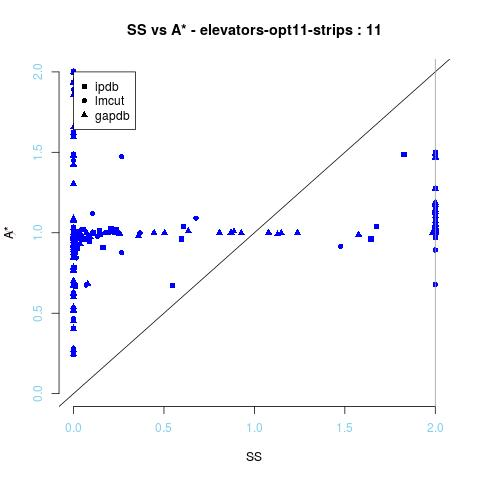
\includegraphics[width=\linewidth]{images/elevators-opt11-strips}
\endminipage\hfill
\minipage{0.32\textwidth}
  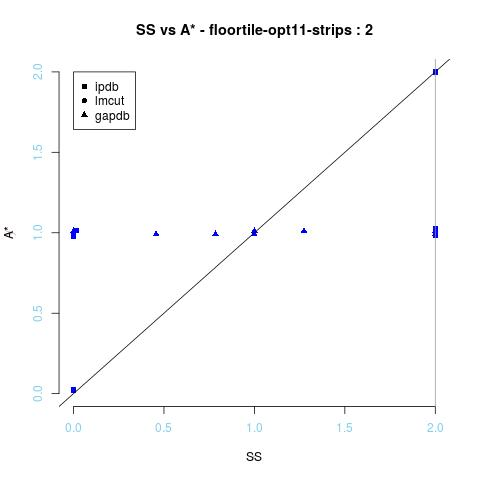
\includegraphics[width=\linewidth]{images/floortile-opt11-strips}
\endminipage\hfill
\minipage{0.32\textwidth}%
  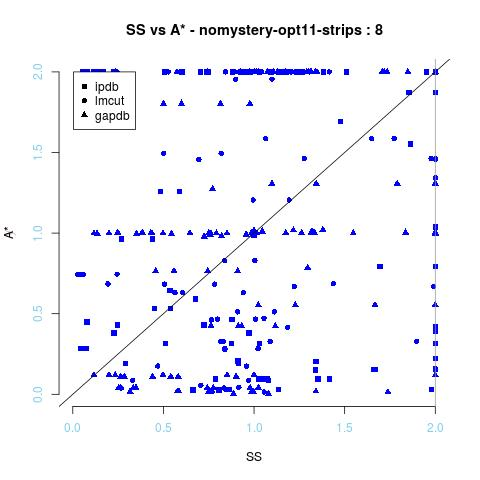
\includegraphics[width=\linewidth]{images/nomystery-opt11-strips}
\endminipage

%jump
\minipage{0.32\textwidth}
  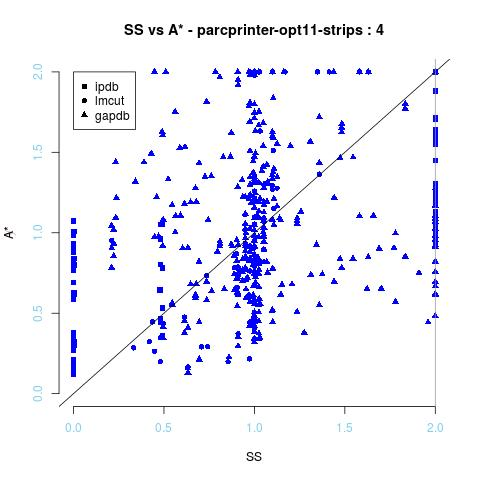
\includegraphics[width=\linewidth]{images/parcprinter-opt11-strips}
\endminipage\hfill
\minipage{0.32\textwidth}
  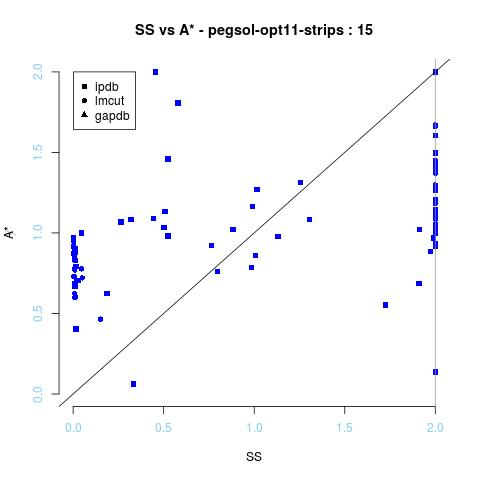
\includegraphics[width=\linewidth]{images/pegsol-opt11-strips}
\endminipage\hfill
\minipage{0.32\textwidth}
  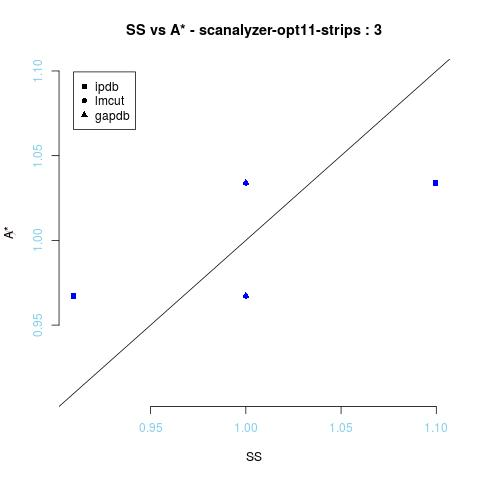
\includegraphics[width=\linewidth]{images/scanalyzer-opt11-strips}
\endminipage\hfill

%jump
\minipage{0.32\textwidth}
  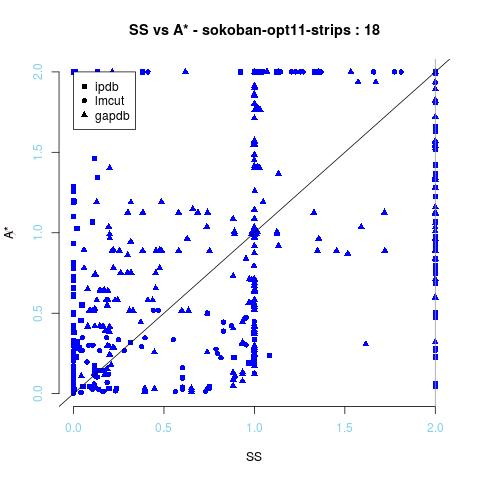
\includegraphics[width=\linewidth]{images/sokoban-opt11-strips}
\endminipage\hfill
\minipage{0.32\textwidth}
  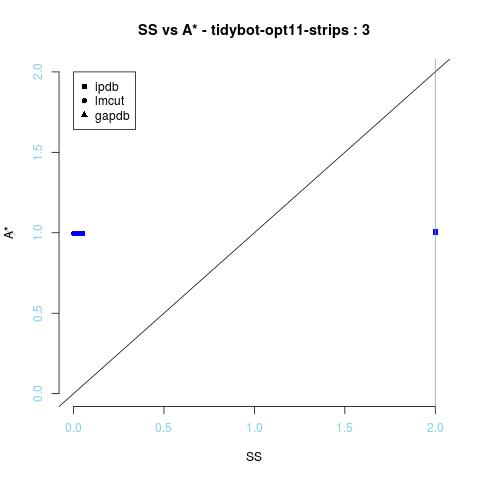
\includegraphics[width=\linewidth]{images/tidybot-opt11-strips}
\endminipage\hfill
\minipage{0.32\textwidth}
  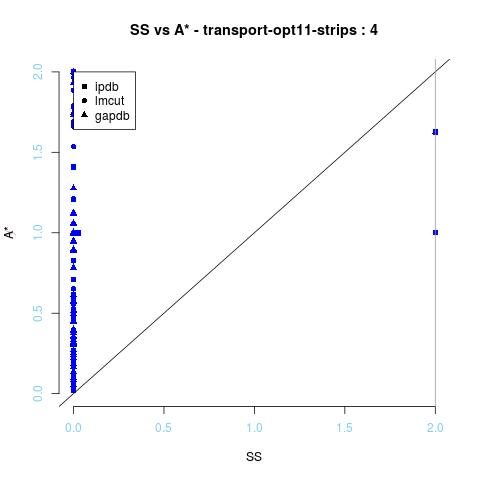
\includegraphics[width=\linewidth]{images/transport-opt11-strips} 
\endminipage\hfill

%jump
\minipage{0.32\textwidth}
  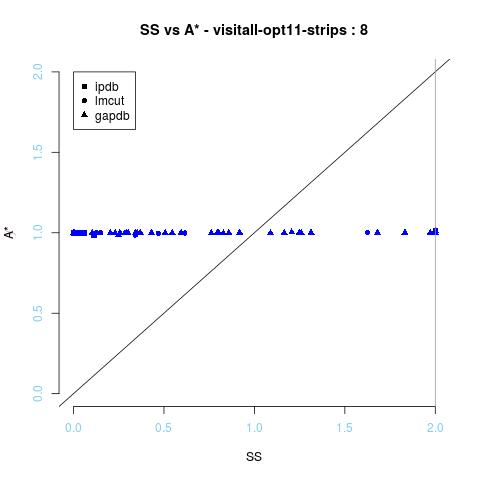
\includegraphics[width=\linewidth]{images/visitall-opt11-strips}
\endminipage\hfill
\minipage{0.32\textwidth}
  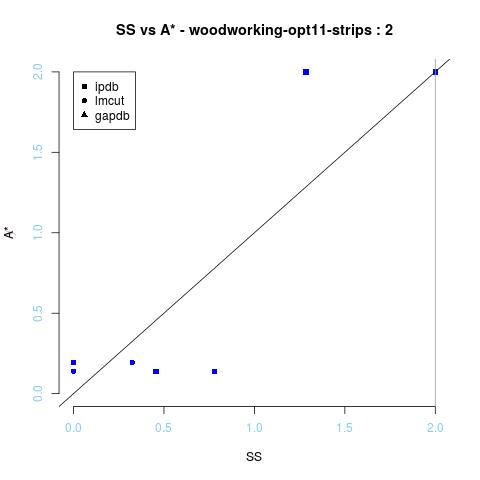
\includegraphics[width=\linewidth]{images/woodworking-opt11-strips}
\endminipage\hfill
\caption{\texttt{SS} vs A$\sp{*}$ ratios for the optimal domains $-$ The number of instances used in each domain are showed next to the name of the Domain.}\label{fig:img_analysis_domains}
\end{figure}

\newpage

In Table \ref{tb:per_ss_made_correctly} we present a single number for each domin representing the percentage of choices \texttt{SS} make correctly. From all the domains all are above of the 50$\%$ which means that at least the half of the points represent good relation of heuristics. With this experiment we prove that \texttt{SS} is not as bad as we thought it would be when we want to make selection.

\begin{table}[!htb]
\centering
\begin{tabular}{lc}
\hline
Domain      & II and III ($\%$) \\ \hline
Elevators   & 78.57    \\
Floortile   & 96.08    \\
Nomystery   & 71.82    \\
Parcprinter & 70.50    \\
Pegsol      & 96.83    \\
Scanalyzer  & 100.00   \\
Sokoban     & 89.31    \\
Tidybot     & 100.00   \\
Transport   & 51.78    \\
Visitall    & 98.05    \\
Woodworking & 100.00   \\ \hline
\end{tabular}
\caption{Percentage of choices \texttt{SS} made correctly.}
\label{tb:per_ss_made_correctly}
\end{table}

\fi

\clearpage